\chapter{The thermal conductivity of strained graphene\label{chap:therm}}

\section{Introduction}
The first measurement of graphene's thermal conductivity was on suspended graphene and was reported to have the highest thermal conductivity ever measured \cite{Balandin2008}.
Shortly thereafter a more modest value with a thermal conductivity roughly one six of the original value was measured for supported graphene \cite{Seol2010}.
This discrepancy has been the source of heavy study in the years since.

The original measurements were performed on suspended graphene samples using an optical technique.
This creative technique uses a laser excitation to heat the sample and the temperature induced energy shift of the Raman scattered light to measure temperature.
In this way a simple Raman measurement serves a dual role as both a heat source and a thermometer.
When used in conjunction with a heat transfer model, this is enough to determine the thermal conductivity.
This technique has advantages and disadvantages.
Uncertainties in the optical absorption and the laser spot size effect the measured thermal conductivity, good results depend on an accurate thermal transport model, and these models are limited by their inability to include ballistic thermal transport.
Nonetheless, the required samples are very simple and the measurement is fairly standard.
This simplicity has resulted in a variety of publications using this technique to study different aspects of thermal transport in suspended graphene \cite{Balandin2008,Faugeras2010,Cai2010,Ghosh2010,Lee2011,Chen2011a,Chen2012}.

The measurement which yielded the more modest values of thermal conductivity were direct measurements of supported graphene.
In these more traditional measurements resistive heaters are used to create a temperature gradient and solid state thermometers are used to measure the temperature.
The thermal conductivity of graphene is then determined directly from the thermal resistance of the graphene.
Although certainly less error prone, there has been only one other measurement of the thermal conductivity of graphene using this technique \cite{Jang2010}.
This is a result of the more difficult measurement and much more difficult sample fabrication.

Figure \ref{fig:therm:lit} summarizes all of the reported room temperature thermal conductivity measurements of single layer graphene.
The thermal conductivity decrease from a value of roughly 2000 W/m-K for suspended graphene to a value close to 500 W/m-K for graphene supported on one side, to a value of less than 160 W/m-K for graphene encased in SiO$_2$ \cite{Jang2010}.
The general observation is that graphene's thermal conductivity is negatively effected by the presence of a supporting or encasing bulk material.
This difference in thermal conductivity is not an artifact of the measurement techniques, a nanoscale thermal conductivity measurement also observed an increase in thermal conductivity for suspended few layer graphene \cite{Pumarol2012}.

\begin{figure}
	\begin{center}
	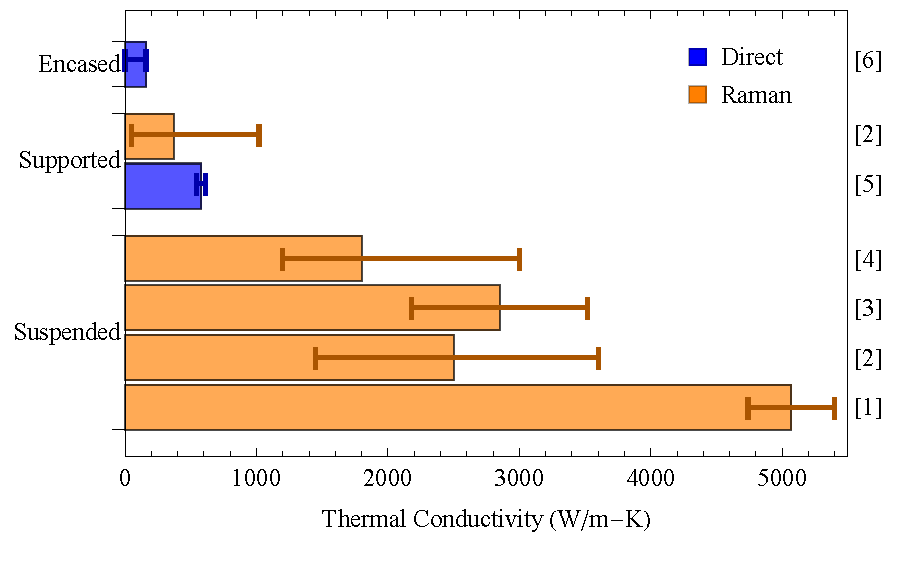
\includegraphics{Figs_Thermal/Thermal_lit.pdf}
	\end{center}
	\caption[Summary of the reported values of the room temperature thermal conductivity of monolayer graphene]{
	\label{fig:therm:lit}
		Summary of the reported values of the room temperature thermal conductivity of monolayer graphene grouped by the environment of the graphene: Suspended, supported on a bulk substrate, and encased in amorphous SiO$_2$ above and below.
		The color code indicates whether the measurements were performed using the Raman technique or a direct technique.
		The number on the right indicate the source: [1] is \cite{Balandin2008}, [2] is \cite{Cai2010}, [3] is \cite{Chen2011a}, [4] is \cite{Lee2011}, [5] is \cite{Seol2010}, [6] is \cite{Jang2010}.
		Error bars are taken from the literature.
	}
\end{figure}

The Raman measurement technique has been advanced in a series of publications.
Faugeras et al was the first to use graphene suspended over a circular aperture.
This circular symmetry of this geometry simplifies the heat transfer model.
Additionally, they used the Raman Stokes to anti-Stokes ratio to measure the temperature and validated the previously used temperature induced phonon energy shift \cite{Faugeras2010}.
Cai et al advanced the thermal transport model by including the thermal transport to the substrate instead of treating supported graphene as a heat sync.
Additionally, they brought up concerns about ballistic thermal transport \cite{Cai2010}.
Chen et al showed that if not accounted for, the thermal conductivity to the gas could inflate the measured value of graphene's thermal conductivity \cite{Chen2011a}.

A variety of potentially interesting physics surrounding the thermal transport of few layer graphene has been studied.
The thickness dependence of the thermal transport has also generated some interest.
Supported graphene's thermal conductivity was shown to converge upward toward graphite's thermal conductivity as the number of layers increased above 34 layers \cite{Sadeghi2013}.
On the other hand the thermal conductivity of suspended graphene was shown to converge downward toward graphite's thermal conductivity as then number of layers increased to four layers \cite{Ghosh2010}.
Ballistic phonon transport has also been of interest.
Since phonons with longer mean free path are able to thermalize and participate in thermal transport for larger samples a size dependence has been expected and observed for trilayer graphene \cite{Wang2010} but not for monolayer CVD graphene \cite{Chen2011a}.
Other studies have concentrated on the effects of scattering on the thermal properties of graphene \cite{Wang2010,Pettes2011,Jang2013,Chen2012}.

\section{Heat transport model}
An accurate heat transport model is necessary for the determination of the thermal conductivity using the Raman measurement technique.
In this section the heat transfer model first proposed by Cai et al is summarized.
It predicts the temperature profile which develops in a circular graphene sealed microchabmer due to central laser heating \cite{Cai2010}.
The temperature profile is then used to predict the anti-Stokes to Stokes ratio following Herman et al \cite{Herman2011}.
Finally, by predicting how the anti-Stokes to Stokes ratio depends on unknown parameters, the importance of the various experimental unknowns is investigated.

The heat transfer model is simplified by the concentric circular symmetry of the laser heating source and the circular microchamber.
The solution is determined by solving the steady state heat equation,
\begin{equation*}
	\vec{\nabla} \cdot \left(\kappa(r) \ \vec{\nabla} T(r) \right) + \dot{Q}=0 \ ,
	\label{eq:therm:heateq}
\end{equation*}
where $T(r)$ is the temperature distribution, $\kappa$ is the thermal conductivity, and $\dot{Q}$ is the generated heat flux per unit time.
The general solution is found by matching the solution for inside, $r<R$, and outside, $r>R$, the edge of the microchamber with boundary conditions at $r=R$.

Isolating the suspended and supported graphene, the generated heat flux includes the laser heating, the energy lost to the gas, and the energy lost to the supporting substrate.
The laser heating is described by,
\begin{align}
	\dot{Q}_{L}=\frac{\alpha P}{t} \frac{1}{2 \pi \sigma^2} e^{-r^2/\sigma^2} \ ,
\end{align}
where $\dot{Q}_L$ is the energy from the incident laser, $P$ is the laser power at the graphene surface, $\alpha$ is the factor of this power which is absorbed by the graphene, $t$ is the thickness of the graphene, $\sigma$ is half the beam waste measured to be 0.81 $\mu$m as shown in Section \ref{sec:fri:Raman}, and $\frac{1}{2 \pi \sigma^2}$ is the normalization factor.
The energy lost to the substrate and gas is modeled using Newton's law of cooling,
\begin{align*}
	\dot{Q}_{S}&=-g_S \frac{1}{t} \left(T(r)-T_0 \right) \\
	\dot{Q}_{g}&=-g_g \frac{1}{t} \left(T(r)-T_0 \right) \ ,
\end{align*}
where $\dot{Q}_{S}$ and $\dot{Q}_g$ are the energy lost to the substrate and to the gas respectively, $g_S$ and $g_g$ are the heat transfer coefficients per unit area, and $T_0$ is ambient temperature.
In the case of the suspended graphene, heat can be lost to both the gas above and below the graphene.
This will be differentiated using $g_g^{\uparrow}$ and $g_g^{\downarrow}$.

When applying Newton's law of cooling for the heat conduction to the silicon dioxide we implicity assume that the temperature of the silicon dioxide remains unchanged.
To test this assumption the thermal oxide is treated as a cylindrical thermal wire connected to a heat sync on one side and with 0.03 mW of power (matching a 1.5 mW laser with 2.3 \% absorption) heating the other side.
The cylinders width was taken to be 200 nm to match the width of the supported graphene that is expected to have elevated temperatures.
An inner radius of 5 $\mu$m, a thickness of 300 nm, and a thermal conductivity of 1.4 W/m-K \cite{} gives a temperature rise of 1.5 K in the thermal oxide.
In the physical system the transport in the silicon dioxide would flare outward resulting in a larger conduction cross section.
Thus, this 1.5 K temperature rise should be treated as an upper bound.
This validates the assumption that the thermal oxide is not significantly heated in our measurements.

Assuming a piecewise uniform thermal conductivity,
\begin{equation*}
	\kappa (\vec{r})=\left \{ \begin{array}{ll} \kappa_{SS} & , r<R \\ \kappa_{SP} & , r \geq R \end{array} \right. \ ,
\end{equation*}
eliminates the spatial dependence of $\kappa$ in the two regions, simplifying the heat equation in Equation \ref{eq:therm:heateq} while still allowing for the disparate suspended and supported thermal conductivities observed in the literature.
While needed to simplify the problem, this simple form for the thermal conductivity may not be entirely accurate. 
A strain dependent thermal conductivity would inherit the spatial dependence of the strain field.
The measurement described here can not provide the spatial information which would inform this more detailed model.
Instead the discussion will be limited to the effective suspended thermal conductivity of the suspended graphene $\kappa_{SS}$.
This factor is a metric which represents the departure of the system from the unstrained case.

Including the generated heat fluxes and the piecewise thermal conductivity in the heat equation, Equation \ref{eq:therm:heateq}, results in two differential equations, 
\begin{equation*}
	\left\{
	\begin{array}{r l}
	\kappa_{SS} \nabla^2 T+\dot{Q}_L + \dot{Q}_g^{\uparrow} + \dot{Q}_g^{\downarrow}=0 & , \textrm{for } r<R \\
	\kappa_{SP} \nabla^2 T+\dot{Q}_S + \dot{Q}_g^{\uparrow}=0 & , \textrm{for } r \geq R
	\end{array}
	\right. \ .
\end{equation*}
In the dimensionless variables
\begin{align*}
	\theta&= \frac{1}{T_a} (T(r)-T_a) \\
	\rho&=\frac{r}{\sqrt{2} \sigma}
\end{align*}
the differential equations become
\begin{equation*}
	\left\{
	\begin{array}{r l}
	\nabla^2 \theta + \beta e^{-\rho^2} - \gamma \theta =0 & , \ \textrm{for } \rho < \frac{R}{\sqrt{2} \sigma} \\
	\nabla^2 \theta - \Gamma \theta =0 & , \ \textrm{for } \rho \geq \frac{R}{\sqrt{2} \sigma}
	\end{array}
	\right. \ , \\
\end{equation*}
where
\begin{align*}
	\beta &=\frac{1}{\pi T_0} \frac{\alpha P}{t \kappa_{SS}}\\
	\gamma&=2 \sigma^2 \frac{g_g^{\uparrow}+g_g^{\downarrow}}{t \kappa_{SS}} \\
	\Gamma&=2 \sigma^2 \frac{g_g^{\uparrow}+g_S             }{t \kappa_{SP}} \ .
\end{align*}

The boundary conditions, 
\begin{align}
	\theta(\infty) &= 0 \label{eq:therm:BC1} \\
	|\theta(0)| &< \infty \label{eq:therm:BC2} \\
	\theta\left(\frac{R}{\sqrt{2} \sigma}\right)^- &= \theta\left(\frac{R}{\sqrt{2} \sigma}\right)^+ 
		\label{eq:therm:BC3} \\
	-\kappa_{SS} \left. \frac{d}{d\rho} \theta^- \right)_{r=\frac{R}{\sqrt{2} \sigma}}&=
	-\kappa_{SP} \left. \frac{d}{d\rho} \theta^+ \right)_{r=\frac{R}{\sqrt{2} \sigma}} \ , \label{eq:therm:BC4}
\end{align}
are written by assuming that the temperature profiles are finite, decay asymptotically to ambient temperature, are continuous at the edge of the microchamber, and have continuous heat flux at the edge of the microchamber respectively.
The heat flux, $\vec{\phi}$, is found using Fourier's law of heat conduction, $\vec{\phi}=-\kappa \vec{\nabla} T(\vec{r})$.

The heat equation for $r \geq R$ has a relatively simple solution.
It can be recast in the form of the modified Bessel's equation and after applying the boundary condition in Equation \ref{eq:therm:BC1} it has the solution,
\begin{equation}
	\theta(\rho)=c_2 K_0 (\sqrt{\gamma} \rho) , \ \textrm{for } \rho \geq \frac{R}{\sqrt{2} \sigma} \ ,
\end{equation}
where $c_2$ is a integration constant and $K_0 (\sqrt{\gamma} \rho)$ is the modified Bessel function of the second kind.

The solution for the suspended graphene is complicated by the incident laser.
Using the substitution $x=\sqrt{\gamma} \rho$ the heat equation can again be cast in the form of a modiffed Bessel function, but this time it is inhomogeneous
\begin{equation*}
	\rho^2 \frac{d^2 \theta}{d x^2}+x \frac{d \theta}{dx}-x^2 \theta = -\frac{\beta}{\gamma}x^2 \ e^{-x^2/\gamma} \ .
\end{equation*}
This differential equation has the general solution
\begin{equation*}
	\theta(\rho)=c_3 I_0(\sqrt{\gamma}\rho) + c_4 K_0(\sqrt{\gamma}\rho) + \theta_P(\sqrt{\gamma} \rho) , \ \textrm{for } \rho \geq \frac{R}{\sqrt{2} \sigma} \ ,
\end{equation*}
where $I_0 (\sqrt{\gamma} \rho)$ is the modified Bessel function of the first kind and $\theta_P (\rho)$ is the particular solution to the inhomogeneous differential equation.
Using the variation of parameters technique, the particular solution can be written as an integral function, 
\begin{align*}
	\theta_P (x)=&\frac{\beta}{\gamma} \left \{
	I_0 (x) \int_0^{x} 
		\frac{K_0(x') \ e^{-x'^2/\gamma} }{-I_0(x') K_1 (x')-K_0(x') I_1 (x')} dx' \right. \\
	&\left.-K_0 (x) \int_0^{x}
		\frac{I_0(x') \ e^{-x'^2/\gamma} }{-I_0(x') K_1 (x')-K_0(x') I_1 (x')} dx'
	\right \} \ .
\end{align*}
Since the particular solution is finite at the origin, the boundary condition in Equation \ref{eq:therm:BC2} requires that $c_4=0$ leaving two integration constants.

These two remaining integration constants are fully determined by the boundary conditions in Equations \ref{eq:therm:BC3} and \ref{eq:therm:BC4}.
This results in two equations with two unknowns,
\begin{align*}
	c_2 K_0(\sqrt{\Gamma/2} R/\sigma)=&c_3 I_0(\sqrt{\gamma/2} R/\sigma)+\theta_P (\sqrt{\Gamma/2} R/\sigma) \\
	c_2 \kappa_{SP} \sqrt{\Gamma} K_1 (\sqrt{\Gamma/2} R/\sigma) =&
		-\kappa_{SS} \sqrt{\gamma} \left \{c_3 I_1(\sqrt{\gamma/2} ) \right. \\
		&+I_1(x) \frac{\beta}{\gamma} \int_0^{x} 
			\frac{K_0(x') \ e^{-x'^2/\gamma} }{-I_0(x') K_1 (x')-K_0(x') I_1 (x')} dx' \\
		&\left.-K_1(x) \frac{\beta}{\gamma} \int_0^{x}
			\frac{I_0(x') \ e^{-x'^2/\gamma} }{-I_0(x') K_1 (x')-K_0(x') I_1 (x')} dx' 	
		\right \}_{x=\sqrt{\frac{\gamma}{2}} \frac{R}{\sigma}} \ ,
\end{align*}
which can be solved for numerically for given $\kappa_{SS}$, $\kappa_{SP}$, $g_g$, and $g_S$.

An example predicted temperature distribution is shown in figure \ref{fig:therm:HTPlot}.
As one might expect, the temperature rise is the greatest where the laser is heating, near the center of the microchamber.
At the edge of the microchamber the slope is discontinuous due to the change in thermal conductivity.
Where the thermal conductivity is lower it takes a larger temperature gradient to conduct the same heat energy.
While the qualitative features of the temperature distribution are simple, the quantitative dependence on the free parameters are non trivial.
The functional dependencies of $\kappa_{SS}$, $\kappa_{SP}$, $g_G$, and $g_S$ are made indecipherable by the form of the particular solution.
The exception is the absorbed power which acts as a linear scaling factor.
Doubling the power simply scales the temperature distribution by a factor of two. 

\begin{figure}
	\begin{center}
	\begin{tikzpicture}[scale=1]

	%The temperature profile
	\node at (0,0) {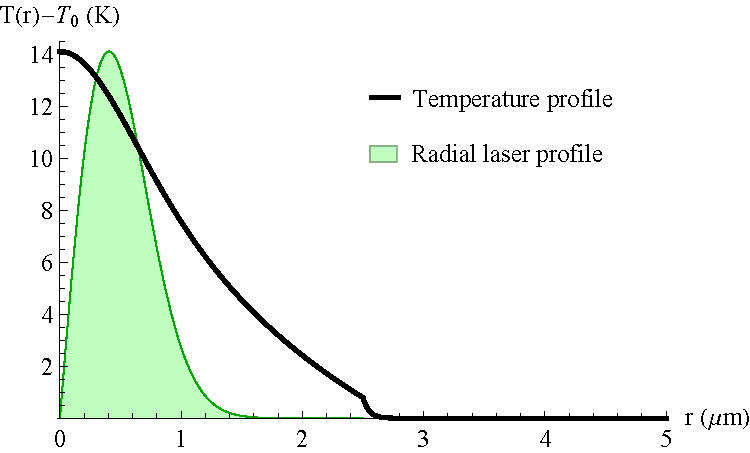
\includegraphics{Figs_Thermal/TemperatureProfile.pdf}};
	
	%The Differential Equations
	\node at (-2.8,-2.25) [fill=white, opacity=.75, text opacity=1,rounded corners=6 pt,inner sep=1.5 pt] {$\kappa_{SS} \nabla^2 T(r) + \dot{Q_L} - \dot{Q_g} =0$};
	\node at (3,-2.25) {$\kappa_{SP} \nabla^2 T(r) - \dot{Q_S} - \dot{Q_g} =0$};
\end{tikzpicture}
	\end{center}
	\caption[Expected temperature distribution in a graphene sealed microchamber heated by a centered laser]
	{\label{fig:therm:HTPlot}
		Theoretical temperature distribution in a graphene sealed microchamber heated by a centered laser.
		The black curve shows the temperature increase for a 5 $\mu$m diameter microchamber assuming that $\kappa_{SS}=2000 \ W/m-K$, $\kappa_{SP}=370 \ W/m-K$, $g_{G}=.03 \ MW/m^2-K$, and $g_{S}=50 \ MW/m^2-K$.
		The radial profile of the 1.5 mW laser heat source with a 0.81 $\mu$m waste is overlaid in green.
		Also shown are the differential equations which govern the heat transfer in the two regions.
	}
\end{figure}